\iffalse
\def\mytitle{PYTHON PROGRAMMING ON MATRICES}
\def\myauthor{Revathi pamujula}
\def\contact{revathipamujula111@gmail.com}
\def\mymodule{Future Wireless Communication (FWC)}


\documentclass[10pt, a4paper]{article}
\usepackage[a4paper,outer=1.5cm,inner=1.5cm,top=1.75cm,bottom=1.5cm]{geometry}

\twocolumn
\usepackage{graphicx}
%\usepackage{karnaugh-map}
\usepackage{tabularx}
\usepackage{hyperref}
\usepackage[utf8]{inputenc}
\usepackage{amsmath}
%\usepackage{physics}
\usepackage{amssymb}
\usepackage{watermark}
\renewcommand*\familydefault{\sfdefault}
\usepackage{lipsum}
\usepackage{xcolor}
\usepackage{listings}
\let\vec\mathbf
\lstset{
frame=single, 
breaklines=true,
columns=fullflexible
}

\begin{document}
\title{\mytitle}
\author{\myauthor\hspace{1em}\\\contact\\FWC22045\hspace{6.5em}IITH\hspace{0.5em}\mymodule\hspace{6em}Matrix:Lines}

%\{ Wireless Communication (FWC)}
\date{}
\maketitle


  \section{Problem}
  \fi
\\
\solution See Fig. 
		\ref{fig:11/10/1/10}.
	\begin{figure}[!ht]
		\centering
 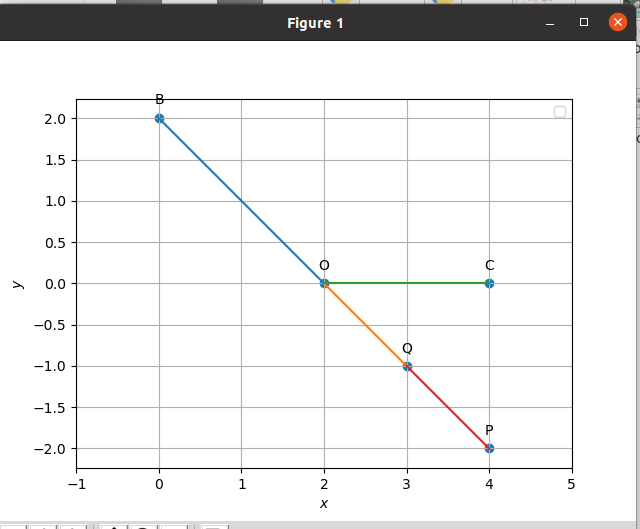
\includegraphics[width=\columnwidth]{chapters/11/10/1/10/figs/fig.png}
		\caption{}
		\label{fig:11/10/1/10}
  	\end{figure}

	\iffalse
\section{Solution}
\textbf{Given that:}
\begin{center}

%\boldmath
	\fi
	Let 
\begin{align}
\vec{P}=\myvec{ 3\\ -1 },
\vec{Q}=\myvec{ 4\\ -2 }
\end{align}
Then 
\begin{align}
	\vec{C}=\vec{P}-\vec{Q}
=\myvec{ -1\\ 1 }
\end{align}
The desired angle is given by
\begin{align}
	\cos\theta&=\frac{\vec{C}^{T}\vec{e}_1}{\norm{\vec{C}}\norm{\vec{e}_1}}
	\\
	&= -\frac{1}{\sqrt{2}}
	\\
	\implies 
	\theta&=135\degree
 \end{align}
 \iffalse
\begin{figure}[h!]
  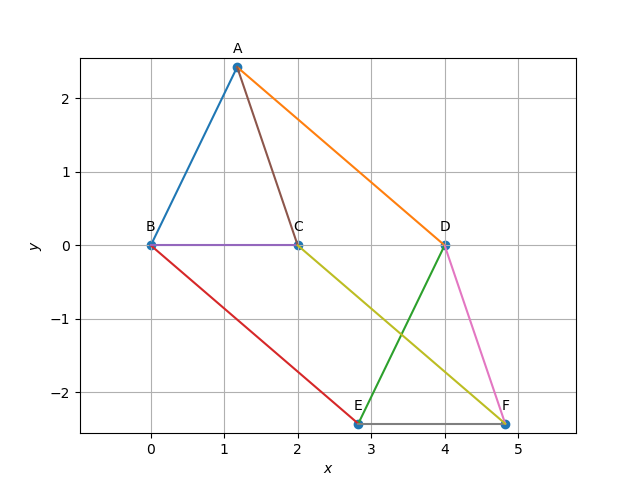
\includegraphics[scale=0.5]{fig.png}
  \caption{line assignment }
  \label{fig:line assignment}
\end{figure}
\end{document}
\fi
